\documentclass{beamer}


\usepackage[utf8]{inputenc}
\usepackage{amsmath}
\usepackage{amsfonts}
\usepackage{amssymb}
\usepackage{graphicx}
\usepackage{ragged2e}  % `\justifying` text
\usepackage{booktabs}  % Tables
\usepackage{tabularx}
\usepackage{tikz}      % Diagrams
\usetikzlibrary{calc, shapes, backgrounds}
\usepackage{amsmath}
\usepackage{amssymb}
\usepackage{dsfont}
\usepackage{url}       % `\url
\usepackage{listings}  % Code listings
\usepackage[T1]{fontenc}
\usepackage[percent]{overpic}
\usetikzlibrary{trees}
\usepackage[absolute,overlay]{textpos}
\usepackage{tcolorbox}



\newtcolorbox{terminal}{colback=black!70!white,colframe=black!70!white}
\newtcolorbox{focus}{colback=black!10!white,colframe=black!10!white}
\newtcolorbox{terminal2}[1]{colback=white,colframe=black!70!white,fonttitle=\bfseries,title=#1}

\usepackage{theme/beamerthemehbrs}

\author[MAS]{Hassan Umari}
\title{ROS Nodes, Topics, and Messages}
\subtitle{Foundation Course}
\institute[HBRS]{Hochschule Bonn-Rhein-Sieg}
\date{\today}
\subject{ROS workshop}

% \thirdpartylogo{path/to/your/image}


\begin{document}
{
\begin{frame}
\titlepage
\end{frame}
}


\section{Recap}
\begin{frame}{Recap}
    \framesubtitle{Summary of yesterday's session}
    \begin{itemize}
        \item ROS is a collection of libraries and tools that helps you when you develop software for robots.
              
        \item ROS provides several ways to transfer data between nodes:
        
        \begin{enumerate}
            \item ROS topics and messages (\textbf{publish/subscribe}).
            \item ROS services (\textbf{request/reply}).
            \item ROS actions (\textbf{request/reply}).
            \item Parameter server.
        \end{enumerate}   
    \end{itemize}
\end{frame}


\begin{frame}{Recap}
    \framesubtitle{Summary of yesterday's session}
    \begin{itemize}
        \item We will focus today on ROS topics and messages..
    \end{itemize}
\end{frame}


     \begin{frame}[plain]{}
         \centering
         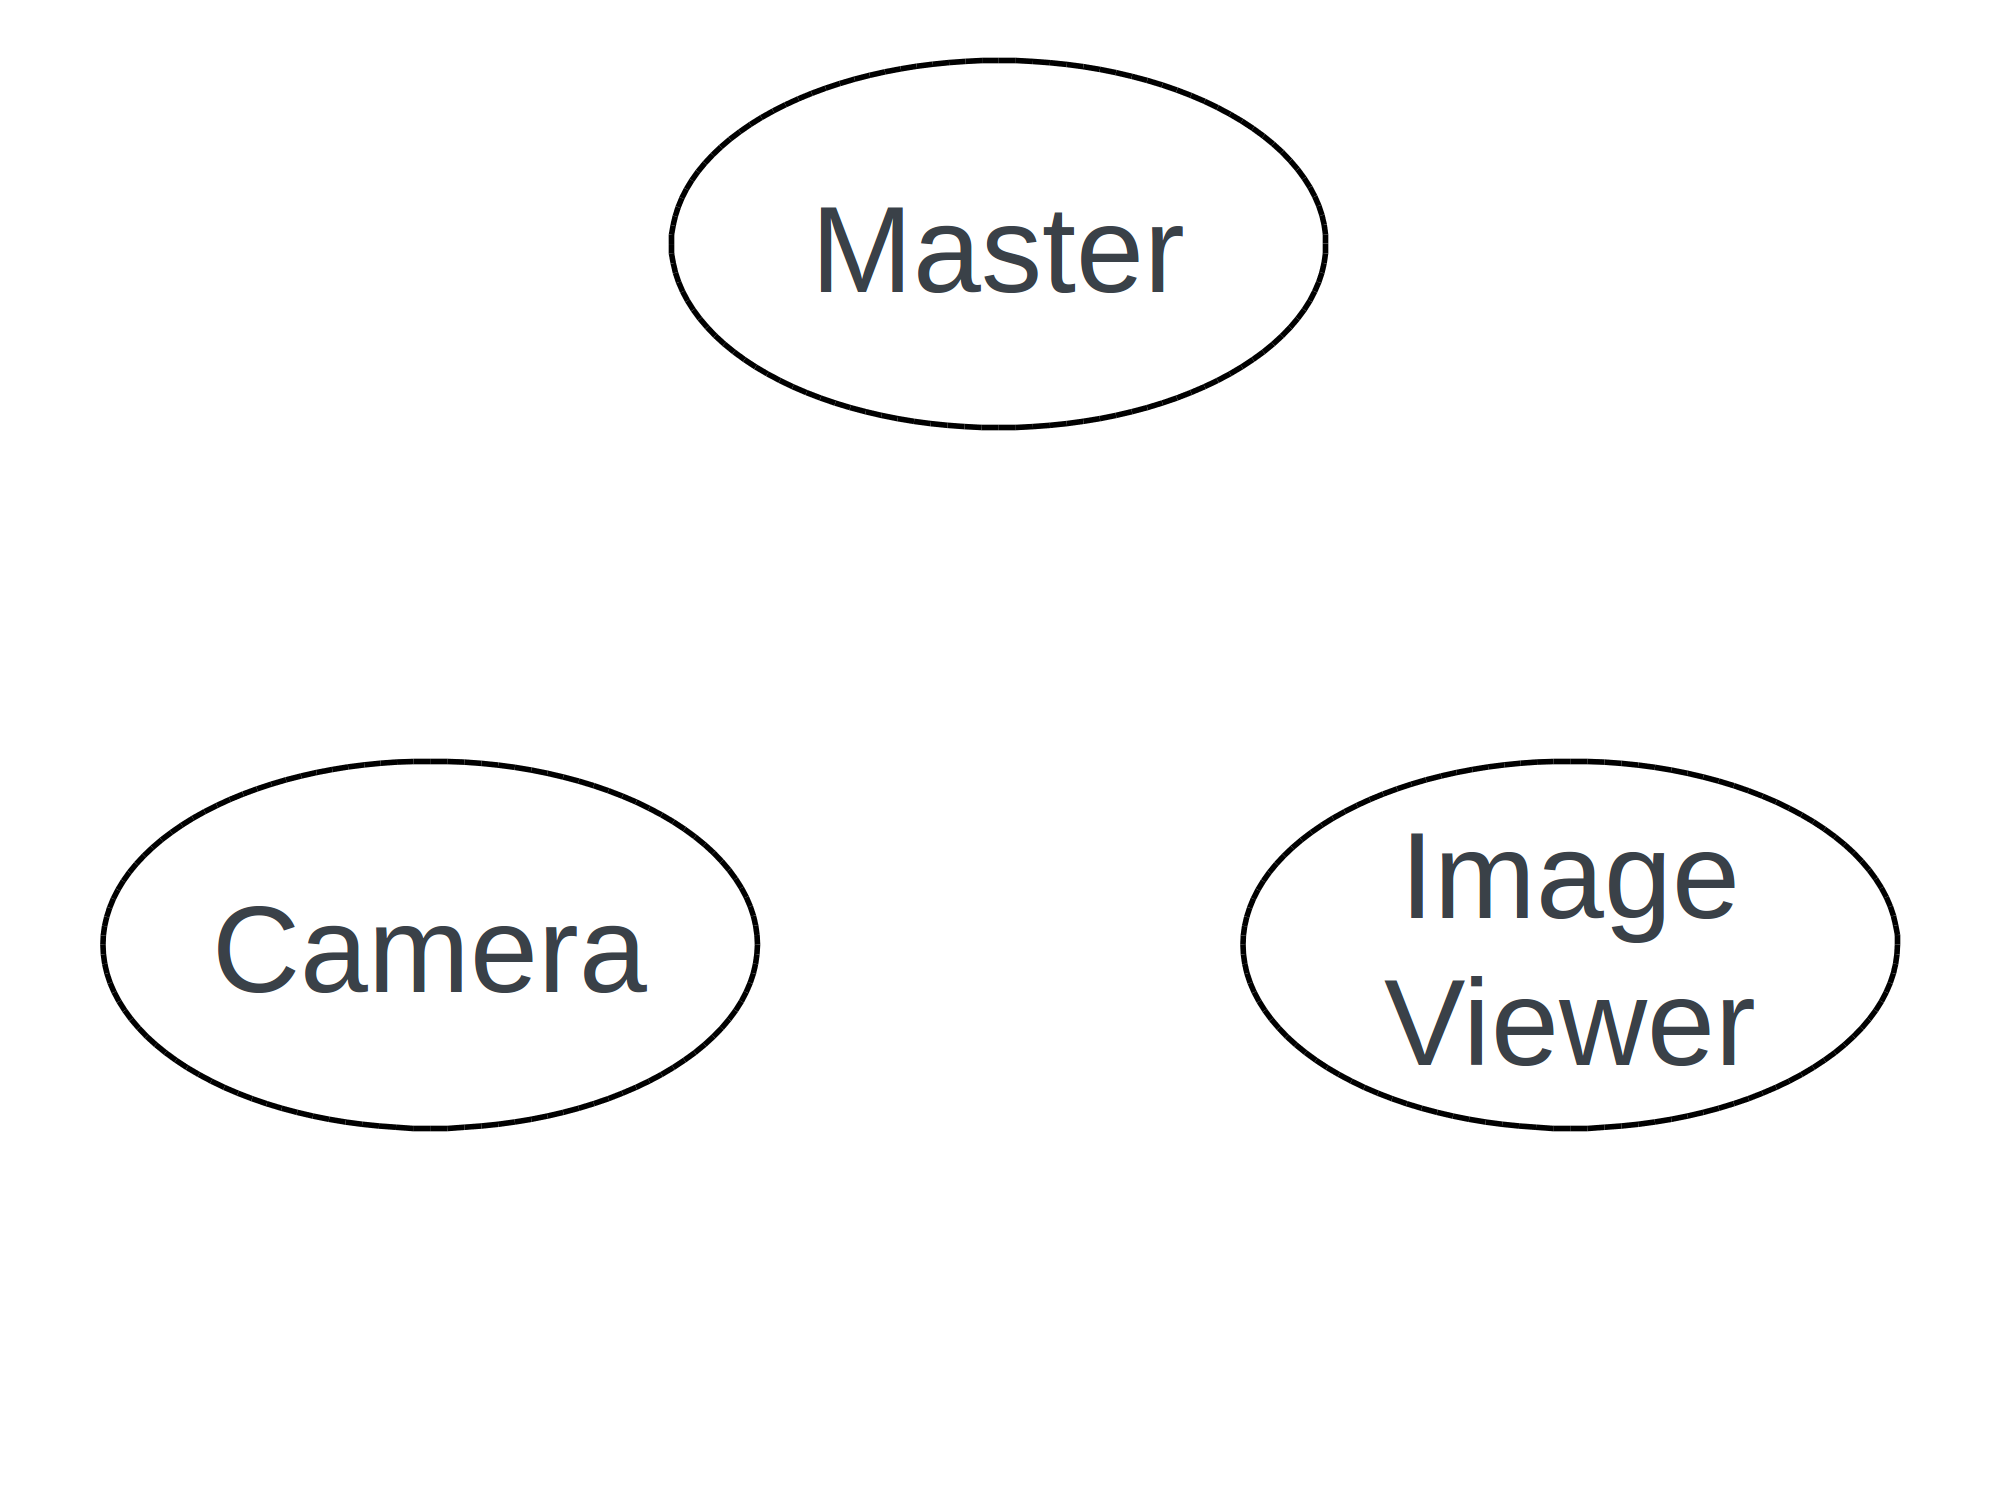
\includegraphics[width =1.0\linewidth]{figures/master1.png}                                                              
        \end{frame} 
        \begin{frame}[plain]{}
            \centering
            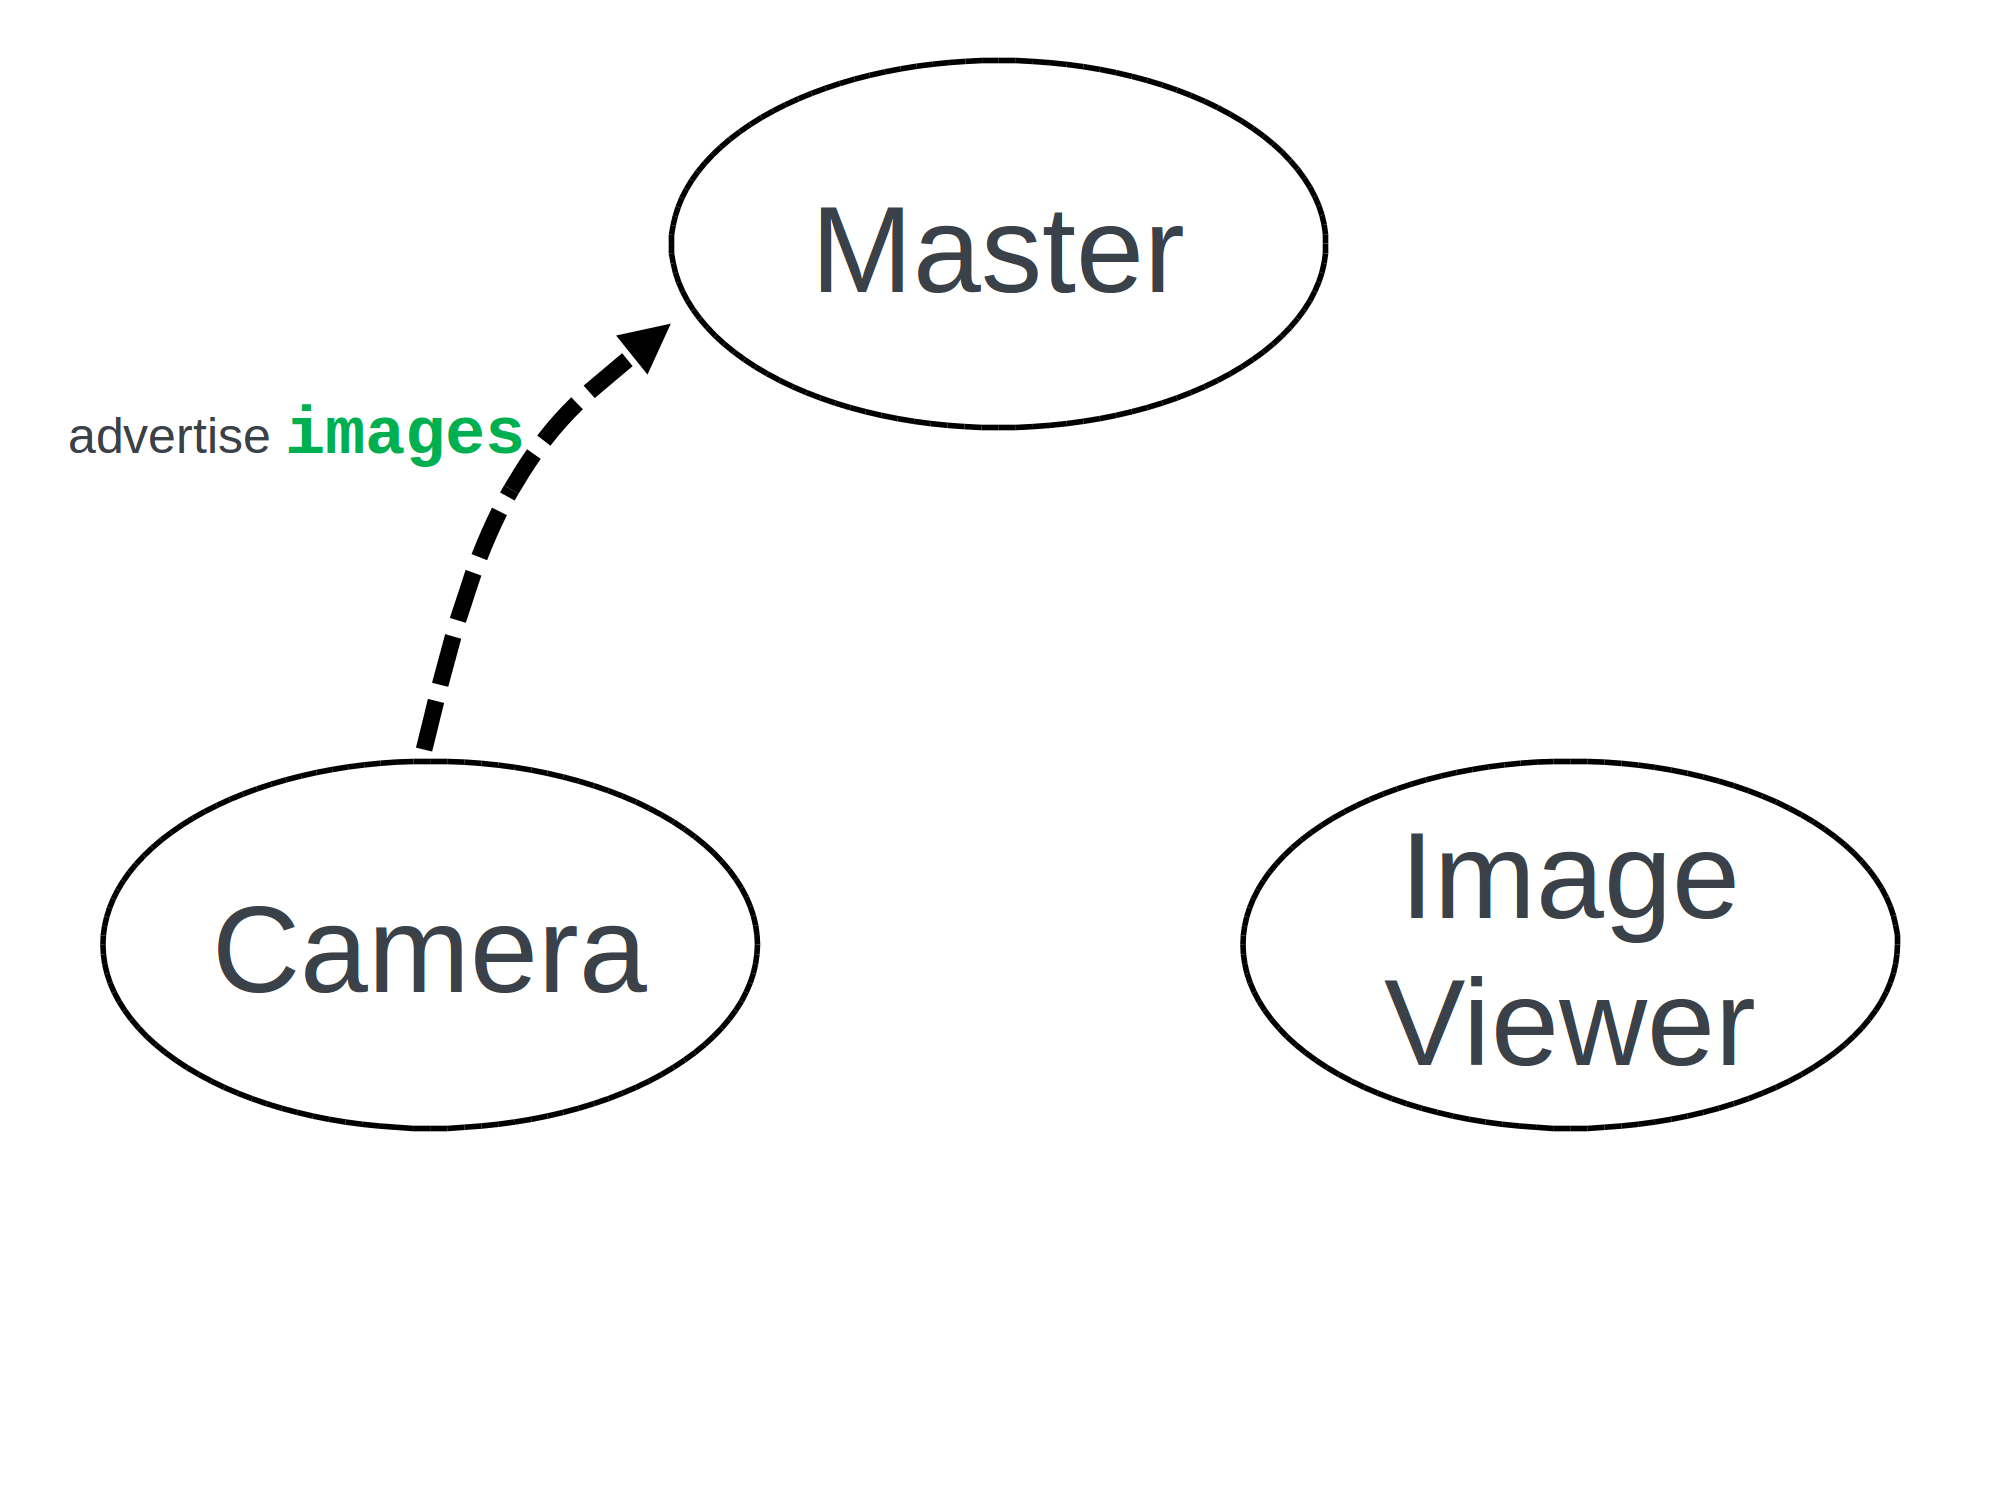
\includegraphics[width =1.0\linewidth]{figures/master2.png}                                                              
        \end{frame} 
        \begin{frame}[plain]{}
            \centering
            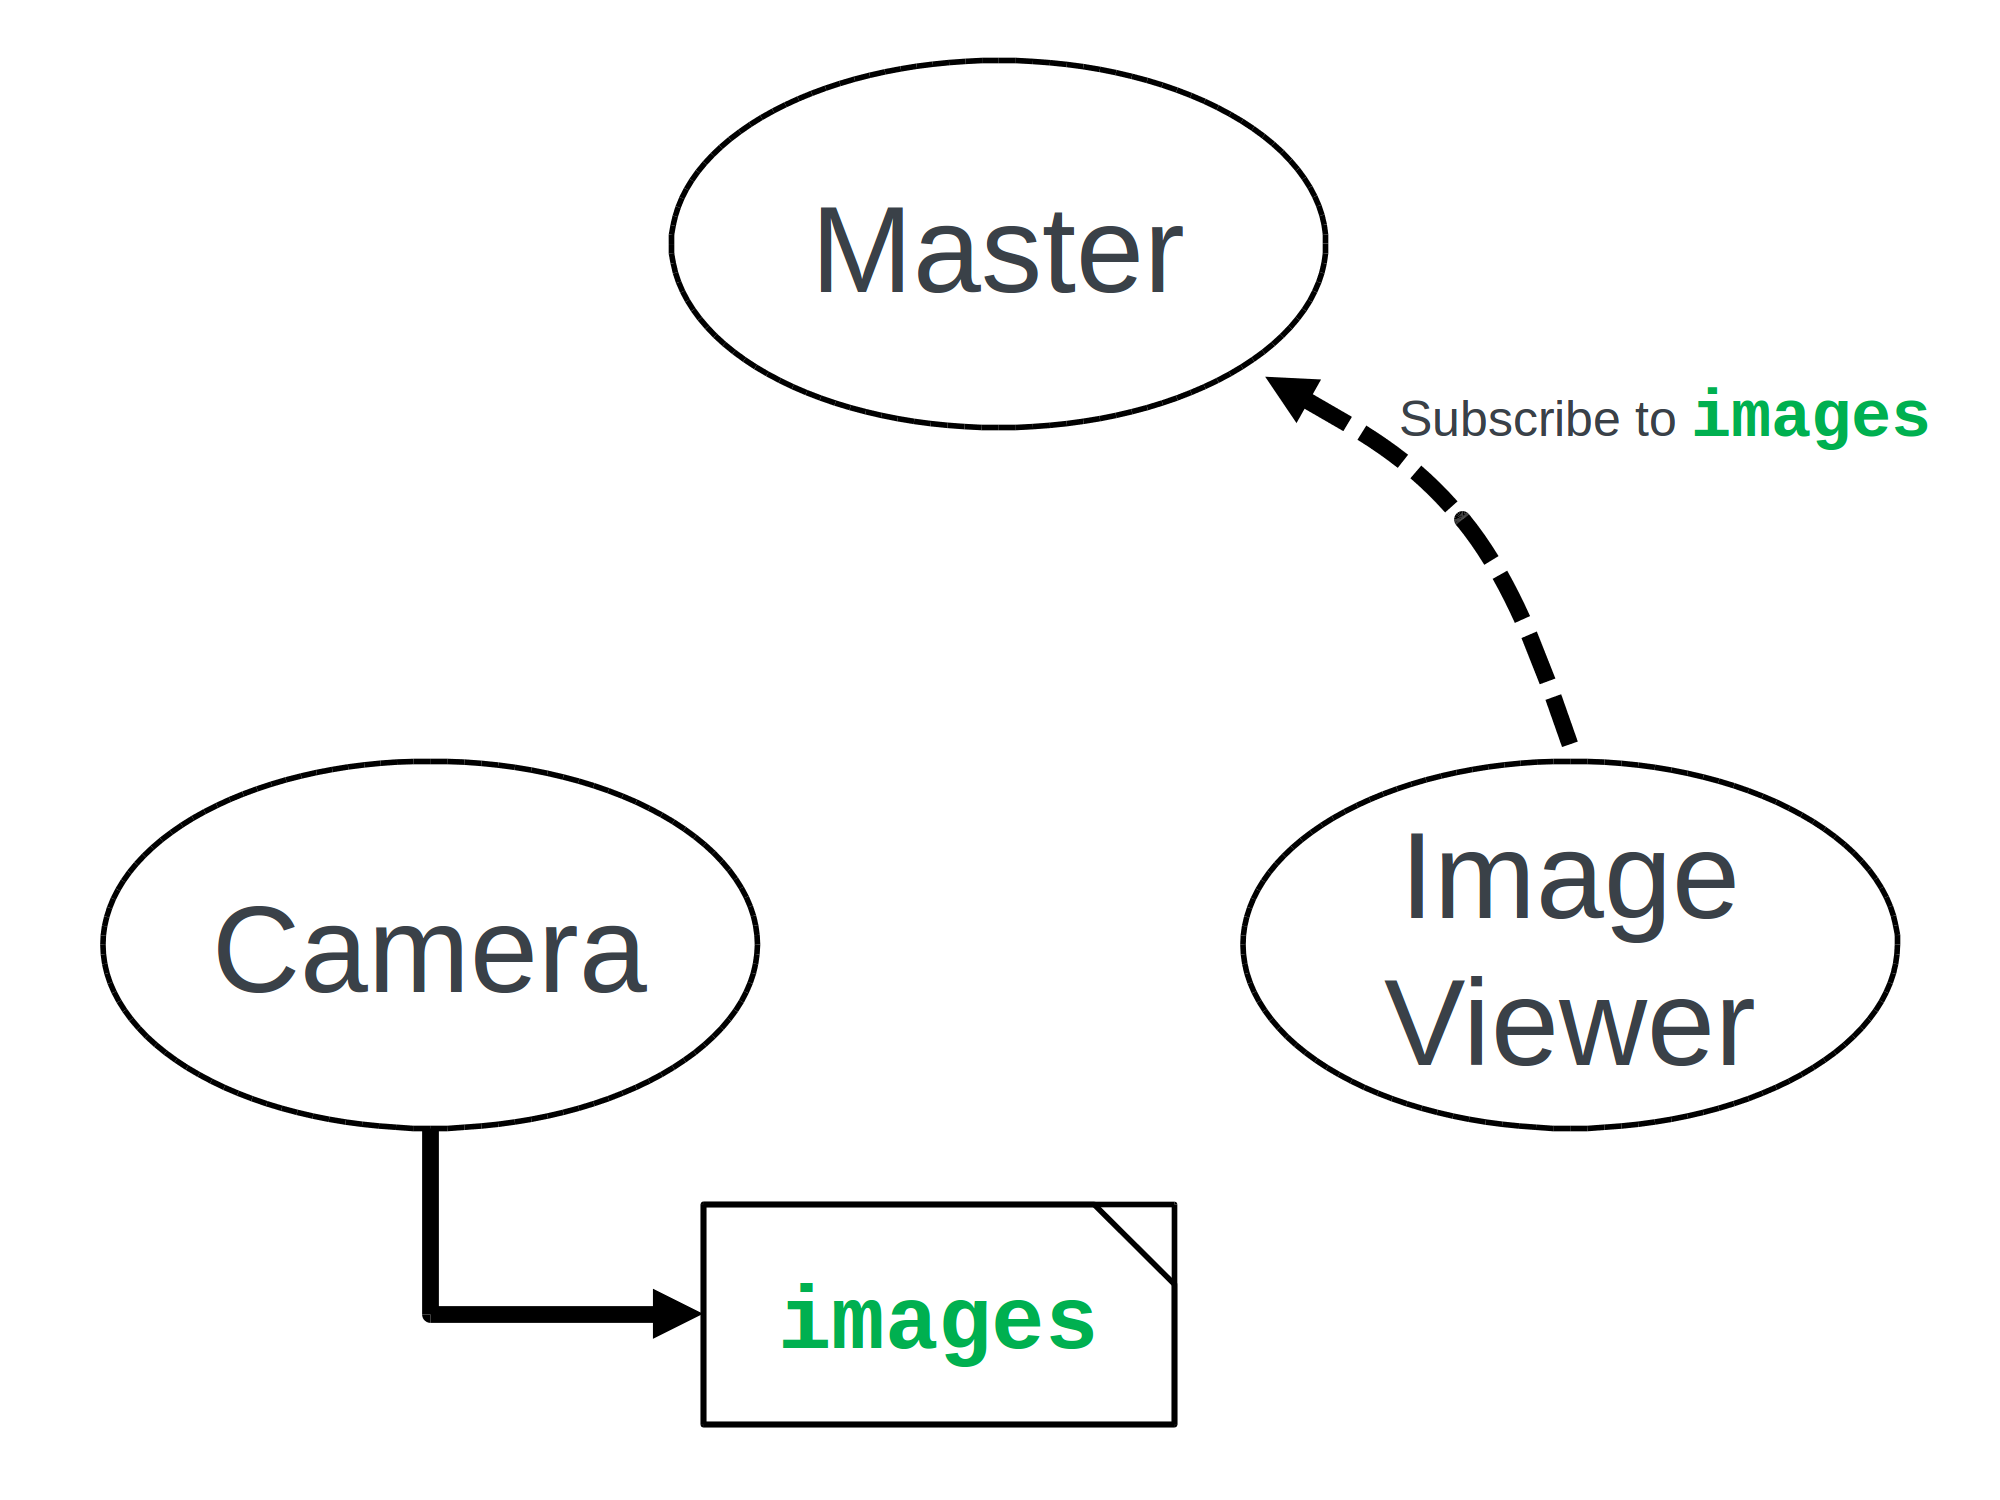
\includegraphics[width =1.0\linewidth]{figures/master3.png}                                                              
        \end{frame} 
        \begin{frame}[plain]{}
            \centering
            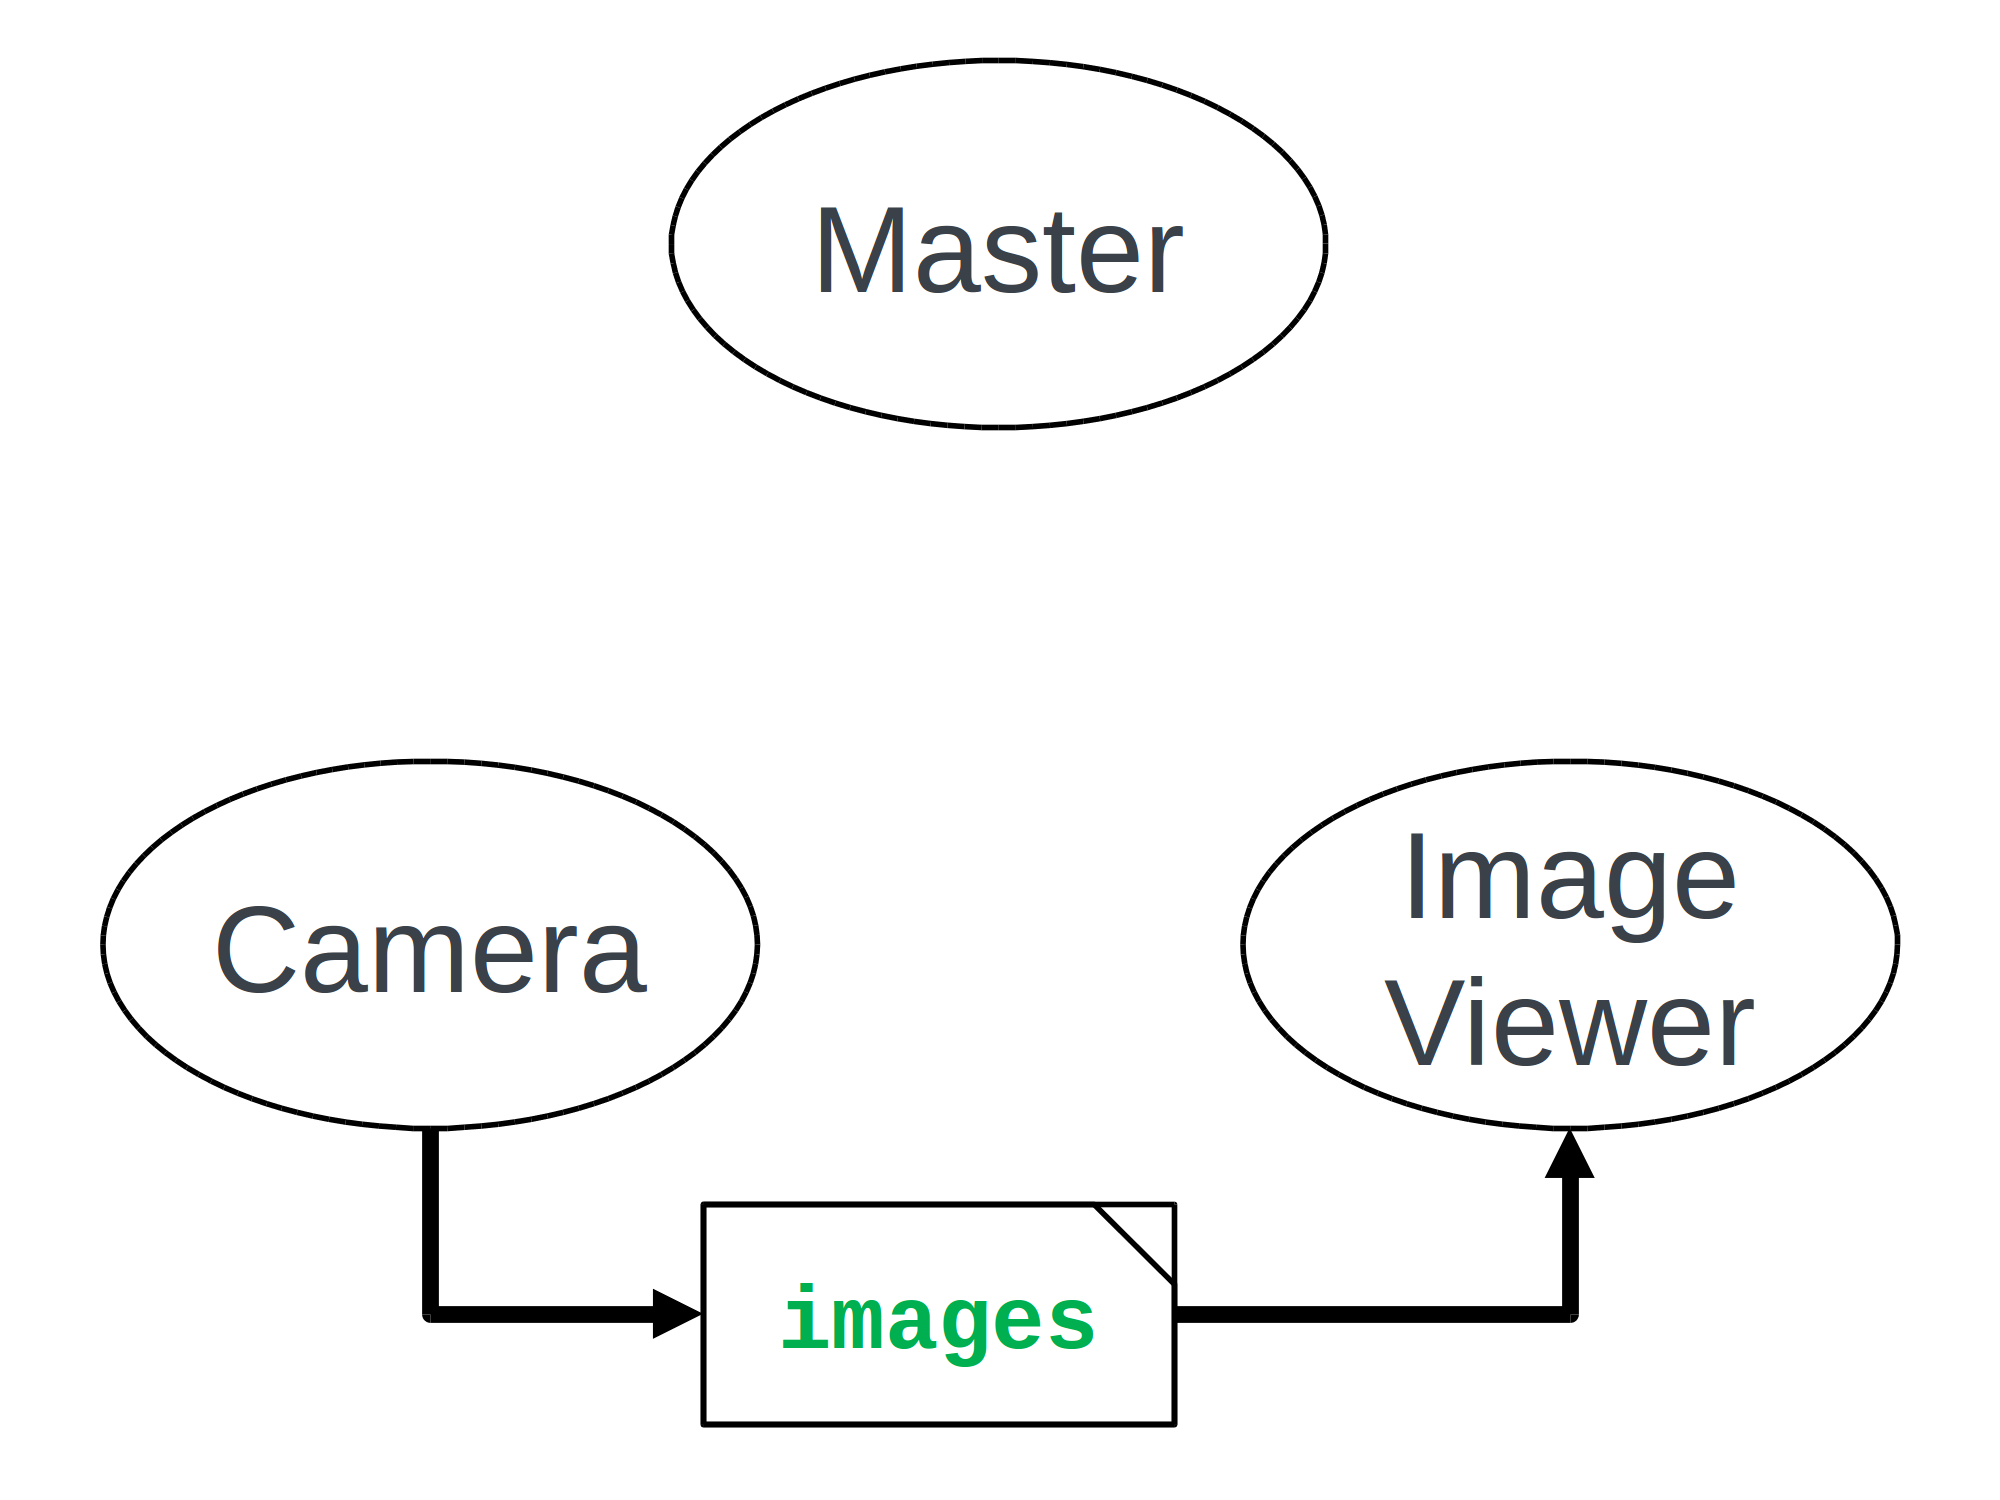
\includegraphics[width =1.0\linewidth]{figures/master4.png}                                                              
        \end{frame}
        
        

        
\section{ROS nodes in Python}

\subsection{A simple ROS node in Python}

\begin{frame}[fragile]{A simple ROS node}
    \framesubtitle{   ../scripts/00\_simple\_node.py}
    \lstset{language=python,
        basicstyle=\ttfamily,
        keywordstyle=\color{blue}\ttfamily,
        stringstyle=\color{red}\ttfamily,
        commentstyle=\color{green}\ttfamily,
        morecomment=[l][\color{magenta}]{\#},
        showstringspaces=false
    }
    \begin{lstlisting}
#!/usr/bin/env python


import rospy
from time import sleep

rospy.init_node("print_text")


while True:
    print "Hello world!"
    sleep(1)
    \end{lstlisting}
\end{frame}



\begin{frame}[fragile]{A simple ROS node}
    \framesubtitle{   ../scripts/01\_simple\_node.py}
    \lstset{language=python,
        basicstyle=\ttfamily,
        keywordstyle=\color{blue}\ttfamily,
        stringstyle=\color{red}\ttfamily,
        commentstyle=\color{green}\ttfamily,
        morecomment=[l][\color{magenta}]{\#},
        showstringspaces=false
    }
\begin{lstlisting}
#!/usr/bin/env python

import rospy


rospy.init_node("print_text")  
rate = rospy.Rate(1)

while not rospy.is_shutdown():
    print "Hello world!"
    rate.sleep()
\end{lstlisting}
\end{frame}



\begin{frame}[fragile]{Writing a publisher node in Python}
    \framesubtitle{../scripts/02\_simple\_publisher.py}
    \begin{focus}
        \centering
        \fontsize{9}{1} \ttfamily rospy.init\_node({\color{blue}'node name'})
    \end{focus}
    
    \begin{itemize}
        \item nodes name must be unique. If you want to make sure the name of the node is unique:
        
        
        \begin{focus}
            \centering
            \fontsize{9}{1} \ttfamily rospy.init\_node({\color{blue}'node name'}, anonymous= {\color{blue}True})
        \end{focus}
        \item node name will look like this: \ttfamily /print\_text\_19637\_1567065017476
    \end{itemize}
    
\end{frame}



\begin{frame}{Three ways to run a node}
    \framesubtitle{ROS Nodes}
    
    There are 3 ways to run a node:
    \begin{enumerate}
        \item Like you normally do {\tiny{(not recommended)}}. Example (in case of python node):
                \begin{terminal}
                \color{green} \ttfamily{python <file name>}
                \end{terminal}
        \item using rosrun command:
        \begin{terminal}
        \color{green} \ttfamily{rosrun <package name> <node name>}
        \end{terminal}
        
        \item Using launch files. \tiny{(we'll see it later)}

    \end{enumerate}
\end{frame}

\begin{frame}{Let's create a package first!}
    \framesubtitle{ROS Nodes}
\begin{itemize}
    \item ROS commands find your files (python scripts, cpp files, launch files, message definitions) if they are located in a package inside the workspace.
    
    \item Normally, a package looks like this:
 
\end{itemize}

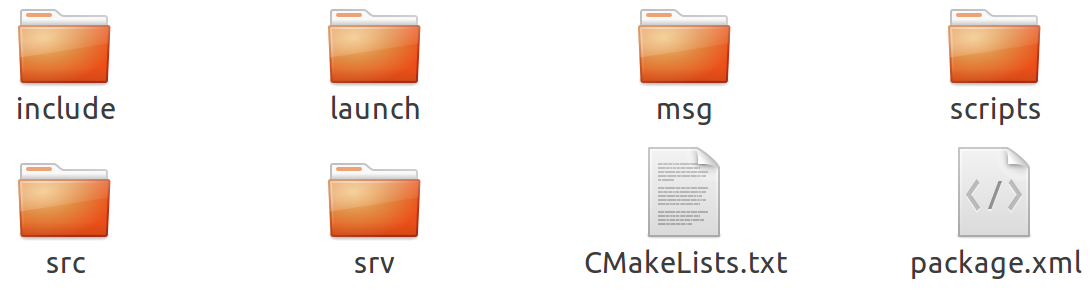
\includegraphics[width = 1\linewidth]{figures/package.png}

\end{frame}

\begin{frame}{Let's create a package first!}
    \framesubtitle{ROS Nodes}

    \begin{itemize}
        \item  go to the README and do the steps for \textbf{creating a package}. 
    \end{itemize}   
\end{frame}


\begin{frame}{ROS commands}
    \framesubtitle{ROS Nodes}
\begin{itemize}
    \item Navigate to a ROS package directly:

    \begin{terminal}
        \color{green} \ttfamily{roscd <package name>}
    \end{terminal}
    
    \item run a node without navigating to it's directory:

    \begin{terminal}
        \color{green} \ttfamily{rosrun <package name> <executable>}
    \end{terminal}
\end{itemize}

\end{frame}


\begin{frame}{Let's create a package first!}
    \framesubtitle{ROS Nodes}
    
    \begin{itemize}
        \item  go to the README and do the steps for \textbf{running a node}. 
    \end{itemize}   
\end{frame}


\begin{frame}{More ROS commands}
    \framesubtitle{ROS Nodes, Topics, and Messages}
    \begin{itemize}
        \item List all the running nodes:
        
        \begin{terminal}
            \color{green} \ttfamily{rosnode list}
        \end{terminal}
        
        \item Get more info. about a certain node:
        
        \begin{terminal}
            \color{green} \ttfamily{rosnode info <node name>}
        \end{terminal}
        
              
        
    \end{itemize}
    
\end{frame}


\subsection{Writing a publisher node in Python}

\begin{frame}[fragile]{Writing a publisher node in Python}
    \framesubtitle{ROS Nodes, Topics, and Messages}
    
    \begin{itemize}
        \item  Let's extend our previous node and make it publish a String ROS message.
    \end{itemize}   
\end{frame}
 
\begin{frame}[fragile]{Writing a publisher node in Python}
    \framesubtitle{../scripts/02\_simple\_publisher.py}
    

                   
    \lstset{language=python,
        basicstyle=\scriptsize,
        keywordstyle=\color{blue}\ttfamily,
        stringstyle=\color{red}\ttfamily,
        commentstyle=\color{green}\ttfamily,
        morecomment=[l][\color{magenta}]{\#},
        showstringspaces=false
    }
\begin{lstlisting}
#!/usr/bin/env python

import rospy

from std_msgs.msg import String

rospy.init_node('talker')

pub = rospy.Publisher('myFirstTopic', String, queue_size=10)

rate = rospy.Rate(1)

my_message = String()
my_message.data = "Hello there! How are you?"

while not rospy.is_shutdown():
    pub.publish(my_message)
    rate.sleep()
\end{lstlisting}
\end{frame}




\begin{frame}[fragile]{Writing a publisher node in Python}
    \framesubtitle{../scripts/02\_simple\_publisher.py}
    \begin{focus}
        \centering
        \fontsize{9}{1} \ttfamily rospy.Publisher({\color{blue}name}, {\color{blue}data\_class}, {\color{blue}queue\_size})
    \end{focus}
    
    \begin{itemize}
        \item {\ttfamily name}: Name of the topic to publish on.
        
        \item {\ttfamily data\_class}: The type of message. It is a ROS message class.
        
        \item {\ttfamily queue\_size}: The size of the outgoing message queue.
        
    \end{itemize}
\end{frame}

\begin{frame}[fragile]{Writing a publisher node in Python}
    \framesubtitle{../scripts/02\_simple\_publisher.py}
    \begin{focus}
        
        \ttfamily rospy.Publisher(\\
                                 {\color{red}name},\\
                                 {\color{red}data\_class},\\
                                 {\color{blue}subscriber\_listener=None}, \\
                                 {\color{blue}tcp\_nodelay=False},\\
                                 {\color{blue}latch=False},\\
                                 {\color{blue}headers=None},\\
                                 {\color{red}queue\_size=None}\\)
    \end{focus}

\end{frame}


\begin{frame}[fragile]{Writing a publisher node in Python}
    \framesubtitle{Things to note..}
    
    \begin{itemize}
        \item  ROS messages are implemented as classes.
        \item  To publish a message you also need to define a \textbf{Publisher} class.
        \item Most of ROS concepts and functionalities are implemented as classes. This is why understanding OOP helps you understand ROS better.
    \end{itemize}   
\end{frame}


\begin{frame}[fragile]{Writing a publisher node in Python}
    \framesubtitle{ROS Nodes, Topics, and Messages}
    
    \begin{itemize}
        \centering
        \item  Go to the README file and do the instructions of section: \textbf{some of ROS commands}.
    \end{itemize}   
\end{frame}




\begin{frame}{More ROS commands}
    \framesubtitle{ROS Nodes, Topics, and Messages}
    \begin{itemize}
        \item Get the current list of topics:
        
        \begin{terminal}
            \color{green} \ttfamily{rostopic list}
        \end{terminal}
        
        \item Print published messages:
        
        \begin{terminal}
            \color{green} \ttfamily{rostopic echo <topic name>}
        \end{terminal}
        
     \end{itemize}
     
\end{frame}


\begin{frame}{More ROS commands}
    \framesubtitle{ROS Nodes, Topics, and Messages}
    \begin{itemize}
                
        \item Publish a message from terminal:
        
        \begin{terminal}
            \color{green} \ttfamily{rostopic pub <topic name> <msg type> <msg>}
        \end{terminal}        
        
        
        \item Get message type of a topic:
        
        \begin{terminal}
            \color{green} \ttfamily{rostopic type <topic name>}
        \end{terminal}
  
  
    \end{itemize}
    
\end{frame}




\subsection{How to use ROS messages}

\begin{frame}{How to use ROS messages}
    \framesubtitle{ROS Nodes, Topics, and Messages}
    \begin{itemize}
        \item ROS messages are just classes with attributes you can fill.
        
        \item ROS messages are defined in separate files and have to be placed in a package. (will be covered today).
        
        \item The following command can be used to see the class attributes, or the description, of a ROS message:
        
        \begin{terminal}
            \color{green} \ttfamily{rosmsg show <package/msg>}
        \end{terminal}
    \end{itemize}
    
\end{frame}


\begin{frame}{How to use ROS messages}
    \framesubtitle{Example}

        \begin{terminal}
            \color{green} \ttfamily{rosmsg show std\_msgs/String }
        \end{terminal}

    The output is:
    
            \begin{terminal}
                \color{green} \ttfamily{string data}
                
            \end{terminal}
   
   \begin{itemize}
       \item It means ROS {\ttfamily \colorbox{yellow}{String}} message is a class with an attribute named {\ttfamily \colorbox{yellow}{data}} of type string (Python string).
   \end{itemize} 
\end{frame}


\begin{frame}{How to use ROS messages}
    \framesubtitle{Importing a ROS message}
    
    
    \begin{itemize}
        \item {\ttfamily \colorbox{yellow}{String}} message is located in the {\ttfamily \colorbox{yellow}{std\_msgs}} package.
    \end{itemize} 
\end{frame}



\begin{frame}[plain]{}
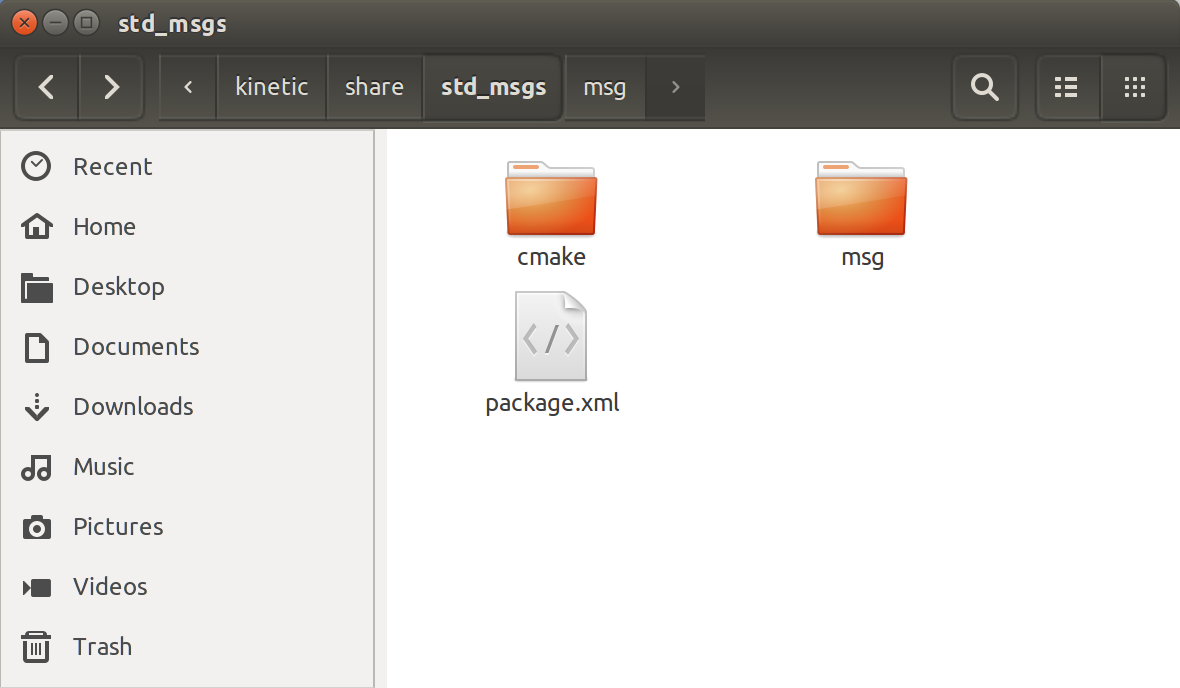
\includegraphics[width=1.0\linewidth]{figures/std_msgs.png}
\end{frame}

\begin{frame}[plain]{}
    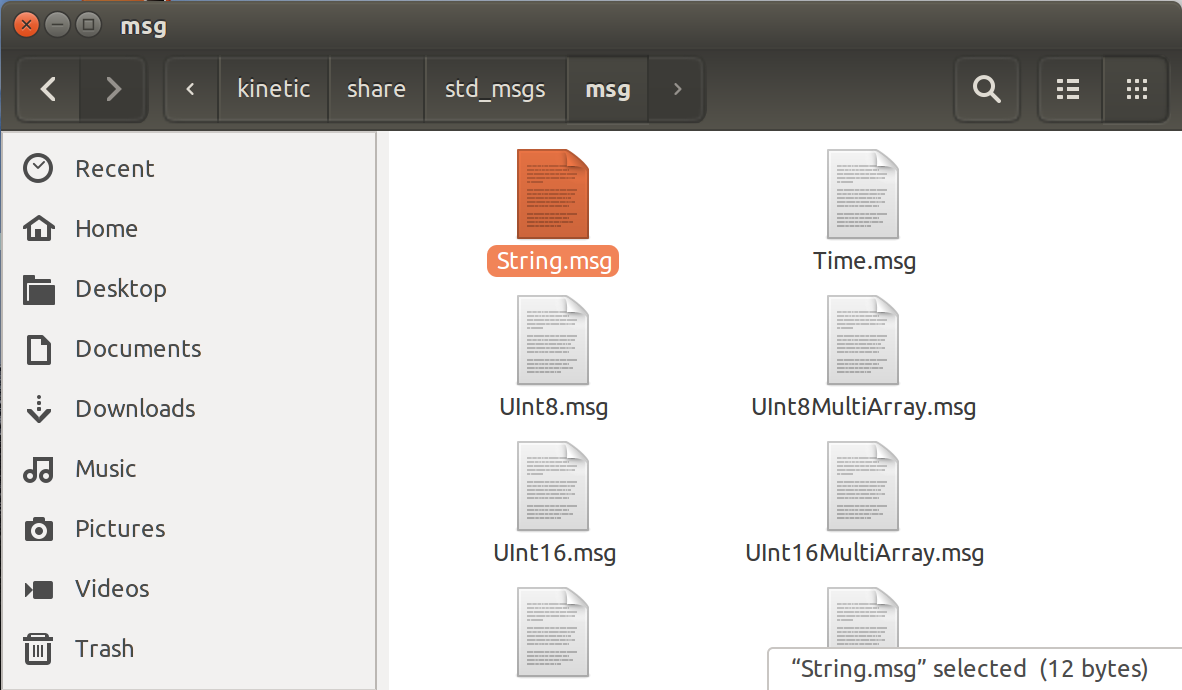
\includegraphics[width=1.0\linewidth]{figures/string.png}
    
    {\scriptsize Note: this is not the file that is imported in our script though! this file is not even Python nor C++. We will see later what this file is.}
\end{frame}




\begin{frame}[fragile]{How to use ROS messages}
    \framesubtitle{Importing a ROS message}
{    \lstset{language=python,
        basicstyle=\ttfamily,
        keywordstyle=\color{blue}\ttfamily,
        stringstyle=\color{red}\ttfamily,
        commentstyle=\color{green}\ttfamily,
        morecomment=[l][\color{magenta}]{\#},
        showstringspaces=false
    }
   
\begin{terminal2}
    {Python}
    \begin{lstlisting}
    from std_msgs.msg import String
    \end{lstlisting} 
\end{terminal2}
}

{	\lstset{language=C++,
        basicstyle=\ttfamily,
        keywordstyle=\color{blue}\ttfamily,
        stringstyle=\color{red}\ttfamily,
        commentstyle=\color{green}\ttfamily,
        morecomment=[l][\color{magenta}]{\#}
    }
\begin{terminal2}
    {C++}
    \begin{lstlisting}
    #include "std_msgs/String.h"
    \end{lstlisting} 
\end{terminal2}
}
\end{frame}


\setbeamercolor{background canvas}{bg=yellow}
\begin{frame}[plain]{}  
    \centering
    {\huge \textcolor{black}{Exercise 1}}
\end{frame}
\setbeamercolor{background canvas}{bg=white}





\subsection{Writing a subscriber node in Python}

\begin{frame}[fragile]{Writing a subscriber node in Python}
    \framesubtitle{../scripts/03\_simple\_subscriber.py}
    \lstset{language=python,
        basicstyle=\scriptsize,
        keywordstyle=\color{blue}\ttfamily,
        stringstyle=\color{red}\ttfamily,
        commentstyle=\color{green}\ttfamily,
        morecomment=[l][\color{magenta}]{\#},
        showstringspaces=false
    }
    \begin{lstlisting}
    
    #!/usr/bin/env python
    
    import rospy
    from std_msgs.msg import String

    def my_callback_function(msg):
        print msg
    
    rospy.init_node('listener')
    rate = rospy.Rate(100) 
    sub = rospy.Subscriber('myFirstTopic', String,
                            callback=my_callback_function)
    
    while not rospy.is_shutdown():
        pass
    
    
    \end{lstlisting}
\end{frame}


\begin{frame}[fragile]{Writing a subscriber node in Python}
        \framesubtitle{../scripts/04\_simple\_subscriber.py}
        
    \lstset{language=python,
        basicstyle=\scriptsize,
        keywordstyle=\color{blue}\ttfamily,
        stringstyle=\color{red}\ttfamily,
        commentstyle=\color{green}\ttfamily,
        morecomment=[l][\color{magenta}]{\#},
        showstringspaces=false
    }
    \begin{lstlisting}
#!/usr/bin/env python

import rospy
from std_msgs.msg import String


def my_callback_function(msg):
    print msg

rospy.init_node('listener')
rate = rospy.Rate(100)

rospy.Subscriber('myFirstTopic', String, callback=my_callback_function)

rospy.spin()

    
    \end{lstlisting}
\end{frame}



\begin{frame}[fragile]{Writing a subscriber node in Python}
    \framesubtitle{Subscriber class}
    
    
    \begin{itemize}
        \centering
        \item go to the README, and let's do section:\\ 
        \textbf{Simple subscriber}
    \end{itemize} 
\end{frame}


\begin{frame}[fragile]{Writing a subscriber node in Python}
    \framesubtitle{Subscriber class}
    \begin{focus}
        
        \ttfamily rospy.Subscriber(\\
        {\color{red}name},\\
        {\color{red}data\_class},\\
        {\color{red}callback=None}, \\
        {\color{blue}callback\_args=None},\\
        {\color{blue}queue\_size=None},\\
        {\color{blue}buff\_size=65536},\\
        {\color{blue}tcp\_nodelay=False}\\)
    \end{focus}
    
\end{frame}




\begin{frame}[fragile]{Writing a subscriber node in Python}
    \framesubtitle{Subscriber class}
    
    
    \begin{itemize}
        \centering
        \item go to the README, and let's do section:\\ 
        \textbf{Simple subscriber}
    \end{itemize} 
\end{frame}


\subsection{General notes}
\begin{frame}{General notes}
    \framesubtitle{more on ROS nodes}
    \begin{itemize}
        \item You can define multiple publishers and subscribers in a node.
        \item You can call {\ttfamily \colorbox{gray!30!white}{init\_node}} function once only!
        \item To make your code look neat, you can wrap ROS stuff in a class and hide them!
    \end{itemize} 
    \vspace{0.5cm}
    Let's see an example with multiple publishers/subscribers and let's define them in a class...
\end{frame}


\setbeamercolor{background canvas}{bg=yellow}
\begin{frame}[plain]{}  
    \centering
    {\huge \textcolor{black}{Let's see script \textbf{05\_node\_example.py}}}
\end{frame}
\setbeamercolor{background canvas}{bg=white}




\section{ROS Launch Files}

\begin{frame}{ROS Launch Files}
    \begin{itemize}
        \item If you are working on a project that is comprised of multiple nodes, it's not practical to run each node manually everytime!
        \vspace{0.4cm}
        \item ROS Launch files provide a way to run/launch multiple nodes at once.
         
    \end{itemize}  
\end{frame}


\begin{frame}[fragile]{ROS Launch Files}
    \framesubtitle{../launch/00\_simple.launch}
    \lstset{language=xml,
        basicstyle=\scriptsize,
        keywordstyle=\color{blue}\ttfamily,
        stringstyle=\color{red}\ttfamily,
        commentstyle=\color{green}\ttfamily,
        morecomment=[l][\color{magenta}]{\#},
        showstringspaces=false
    }
    \begin{lstlisting}
<!-- Example launch file to run the turtlesim node-->

<launch>

<node pkg="turtlesim" type="turtlesim_node" name="turtle"/>

</launch>
    \end{lstlisting}
\end{frame}


\begin{frame}{ROS Launch Files}
    \begin{itemize}
        \item To run a launch file:
             \begin{terminal}
                 \color{green} \ttfamily{roslaunch <package name> <launch file>}
              \end{terminal}
              
        \item Example
        \begin{terminal}
            \color{green} \ttfamily{roslaunch my\_first\_package 00\_simple.launch}
          \end{terminal}              
    \end{itemize}  
\end{frame}


\begin{frame}{ROS Launch Files}
    \begin{itemize}
        \item Ros launch files are XML files that consists for tags.
        
        \item They have {\ttfamily \colorbox{gray!30!white}{.launch}} file extension.
        
        \item You would ideally place them inside a {\ttfamily \colorbox{gray!30!white}{launch}} folder inside your package.
    \end{itemize}  
    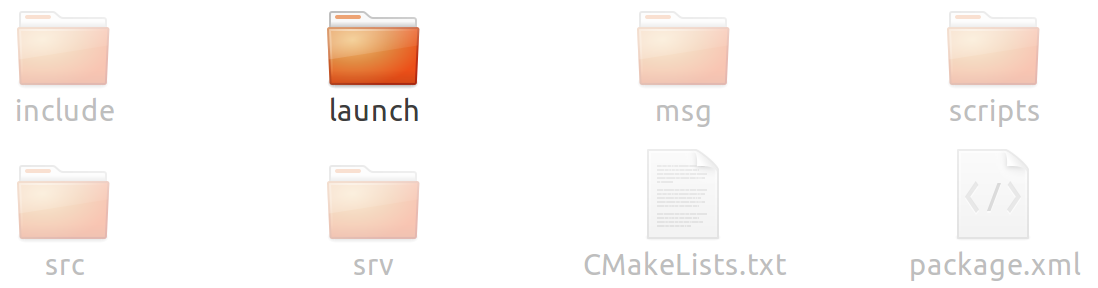
\includegraphics[width=1.0\linewidth]{figures/package2.png}
\end{frame}

\begin{frame}{ROS Launch Files}
    \begin{itemize}        
        \item With launch files, you can do the following:
        \begin{itemize}
            \item Define nodes to be run.
            
            \item Set ROS parameters on the parameter server.
            
            \item Name remapping (will be covered later).
            
            \item Define arguments for the launch file itself.
            
            \item Include other launch files, and pass arguments to them.
            
            \item Bring up the master (no need to call {\ttfamily \colorbox{gray!30!white}{roscore}}).
            
            \item Push a group of nodes into a separate namespace (will be covered later).
           
             \item The list goes on..          
           \end{itemize} 

        
    \end{itemize}  
\end{frame}


\begin{frame}[fragile]{ROS Launch Files}
    \framesubtitle{../launch/01\_simple.launch}
    \lstset{language=xml,
        basicstyle=\scriptsize,
        keywordstyle=\color{blue}\ttfamily,
        stringstyle=\color{red}\ttfamily,
        commentstyle=\color{green}\ttfamily,
        morecomment=[l][\color{magenta}]{\#},
        showstringspaces=false
    }
    \begin{lstlisting}
    <!-- Example launch file to run 
    the turtlesim node and our script 06-->
    
    <launch>
    
    <node pkg="turtlesim" type="turtlesim_node" name="turtle"/>
    
    <node pkg="my_first_package" type="06_parameters_example.py" 
     name="commander"/>
    
    </launch>
    \end{lstlisting}
\end{frame}


\begin{frame}{ROS Launch Files}
    \begin{itemize}
        \centering
        \item Go to the README, and do section  \\   \textbf{Using launch files}
    \end{itemize}  
\end{frame}

\section{Names in ROS}

\section{Parameter Server}

\begin{frame}{Parameter Server}
    \begin{itemize}
        \item A network-shared dictionary accessible to all nodes.
        \item  All nodes can access and modify those values.
        \item Parameter server is a part of ROS Master.
    \end{itemize}  
\end{frame}

\begin{frame}{Parameter Server}
    \framesubtitle{Command line tools}
    \begin{itemize}
        
        \item The {\ttfamily \colorbox{gray!30!white}{rosparam}} command can do the following:
        
        \begin{itemize}
            \item Get a list of parameter names currently held by the master.
            
                    \begin{terminal}
                        \color{green} \ttfamily{rosparam list }
                    \end{terminal} 
            \item Set/change the value of a parameter:
                    \begin{terminal}
                        \color{green} \ttfamily{rosparam set <parameter name>}
                     \end{terminal}   
            
            \item Get/fetch the value of a parameter:
                    \begin{terminal}
                        \color{green} \ttfamily{rosparam get <parameter name>}
                       \end{terminal}                                            
        \end{itemize}
    \end{itemize}
\end{frame}

\begin{frame}{Parameter Server}
    \framesubtitle{rospy interface to the parameter server}
    \begin{itemize}
        
        \item A node can fetch/retrieve a parameter as follows:
        
        
            \begin{focus}
                \centering
                \fontsize{9}{1} \ttfamily rospy.get\_param({\color{blue}param\_name})
            \end{focus}
       \item It can optionally define a default value in case the parameter is not set in the parameter server:
         \begin{focus}
             \centering
       \fontsize{9}{1} \ttfamily rospy.get\_param({\color{blue}param\_name},{\color{blue}default=value})
        \end{focus}
        
       \item A node can set a parameter on the parameter server:
       \begin{focus}
           \centering
           \fontsize{9}{1} \ttfamily rospy.set\_param({\color{blue}param\_name},{\color{blue}param\_value})
        \end{focus}
    \end{itemize}
\end{frame}



\setbeamercolor{background canvas}{bg=yellow}
\begin{frame}[plain]{}  
    \centering
    {\huge \textcolor{black}{Let's see script \textbf{06\_parameters\_example.py}}}
\end{frame}
\setbeamercolor{background canvas}{bg=white}



\begin{frame}{Parameter Server}
    \framesubtitle{Examples}

The examples that follows, assume the node name is {\ttfamily \colorbox{yellow}{move}}  and has a namespace of {\ttfamily \colorbox{yellow}{/robot1}}, so the resolved node name is   {\ttfamily \colorbox{yellow}{/robot1/move}} 

    
\end{frame}


\begin{frame}{Parameter Server}

    \begin{itemize}
        \item Global naming:
        \begin{focus}
            \centering
            \fontsize{9}{1} \ttfamily  var = rospy.get\_param("/speed") \\ \vspace{0.2cm}  resolves to  $\Rightarrow$ {\color{red} /speed}
        \end{focus}
        
        \item Relative naming:
        \begin{focus}
            \centering
            \fontsize{9}{1} \ttfamily var = rospy.get\_param("speed")\\ \vspace{0.2cm}  resolves to  $\Rightarrow$ {\color{red} /robot1/speed}
        \end{focus}  
        
        \item Private naming:
        \begin{focus}
            \centering
            \fontsize{9}{1} \ttfamily var = rospy.get\_param("$\sim$speed")\\ \vspace{0.2cm}  resolves to  $\Rightarrow$ {\color{red} /robot1/move/speed}
        \end{focus}        
        
    \end{itemize}
    
\end{frame}






\section{Catkin and Custom ROS messages}



\subsection{Catkin}


\begin{frame}{Catkin}
    
    \begin{itemize}
        \item In ROS, packages are compiled and built using Catkin.
        
        \item The build process is not only to compile C++ nodes, it's also used to generate source files (ex. Python and C++ files that define ROS messages as classes which you can import/include).
        
        \item Today, we will look at ROS message generation, and how to define custom ROS messages.
        
    \end{itemize}
    \end{frame}
    
    
\begin{frame}{Catkin}
    
    \begin{itemize}
        \item Catkin is not a compiler. It is a tool that handles the compilation process from source files to executables. It invokes system's compiler (ex. g++) and handles your package dependencies.
        
        \item to do that, Catkin needs information on what to compile, where to find, etc...
        
    \end{itemize}
\end{frame}
    

\begin{frame}{A ROS package}
    
    \begin{itemize}
        \item The  {\ttfamily \colorbox{yellow}{CMakeList.txt}} file is what tells Catkin these things.
        
        \item {\ttfamily \colorbox{yellow}{package.xml}} file is where you add information about the package (author, maintainer, dependencies, etc..). 
        
    \end{itemize}
    
    \begin{overpic}[width = 1\linewidth]{figures/package.png}
        \thicklines
        \put(36, 6){\color{red}\circle{13}}
        \put(66, 6){\color{red}\circle{13}  }
    \end{overpic}
    
\end{frame}

\begin{frame}{Catkin}
    
    \begin{itemize}
        \item These files are auto-generated by {\ttfamily \colorbox{yellow}{catkin\_create\_pkg}}  command.
    \end{itemize}

    
\end{frame}


\subsection{Package Manifest}

\begin{frame}{Package Manifest}
    \framesubtitle{package.xml file}
    
    \begin{itemize}
        \item Go to the package we have created earlier ({\ttfamily \colorbox{yellow}{my\_first\_package}}) and open the {\ttfamily \colorbox{yellow}{package.xml}} file there.
    \end{itemize}
   \end{frame} 
   
    
   \begin{frame}{Package Manifest}
       \framesubtitle{package.xml file}
   
        \begin{itemize}
            \item It's an XML file that consists of tags you need to fill.
            
            \item It defines properties of the package which include:
            \begin{itemize}
                \item Name of the package: {\color{red}<name>}.
                \item Version number: {\color{red}<version>}.
                \item Description: {\color{red}<description>}.
                \item Package maintainer: {\color{red}<maintainer>}.
                \item License: {\color{red}<license>}.
                \item Package URL: {\color{red}<url>}.
                \item Author of package {\color{red}<author>}.
            \end{itemize}
        \end{itemize}
    
\end{frame}

   \begin{frame}{Package Manifest}
       \framesubtitle{package.xml file}    
    \begin{itemize}
        \item It also defines package dependencies:
        \begin{itemize}
            \item  Build Dependencies: {\color{red}<build\_depend>}.
            \item Build Export Dependencies: {\color{red}<build\_export\_depend>}.
            \item Execution Dependencies: {\color{red}<exec\_depend>}.
            \item Test Dependencies: {\color{red}<test\_depend>}.
            \item Build Tool Dependencies: {\color{red}<buildtool\_depend>}. (catkin)
            \item Documentation Tool Dependencies: {\color{red}<doc\_depend>}
            \item All of the above: {\color{red}<depend>}.
        \end{itemize}
    \end{itemize}
    
\end{frame}




\subsection{Package Manifest}

\begin{frame}{CMakeLists.txt}
    
    \begin{itemize}
        \item The second file is ({\ttfamily \colorbox{yellow}{CMakeLists.txt}}). This defines how to build the package, what to compile, etc..
        \item Go to the package we have created earlier ({\ttfamily \colorbox{yellow}{my\_first\_package}}) and open the({\ttfamily \colorbox{yellow}{CMakeLists.txt}}).
    \end{itemize}
\end{frame}




\subsection{Custom ROS Messages}




    

\begin{frame}[fragile]{rospy reference}
    \framesubtitle{}

\begin{itemize}
    \item rospy full documentation (all the classes, all the functions ..etc):
    
    \vspace{0.5cm}
     \url{http://docs.ros.org/kinetic/api/rospy/html/}
\end{itemize}
    
\end{frame}





\end{document}
